\documentclass[12pt, a4paper, oneside]{mwart} % Z automatu 10pt w przypisach
\usepackage[utf8]{inputenc} % Znaki diakrytyczne z klawiatury
\usepackage[OT4]{fontenc} % OT4 ponizej nie dzialalo
\usepackage[plmath,MeX]{polski} % Ponoc lepsza polonizacja LaTeXa
%\usepackage[dvips]{graphicx}
\usepackage[pdftex]{color,graphicx} % Grafika w PDFowej formie
%\usepackage{dcolumn} % Wyrownywanie przecinka w tabelach
%\newcolumntype{d}[1]{D{.}{,}{#1}} % Typ kolumny do wyrownywania
%\usepackage{threeparttable} % Coby ladnie podpisac tabelki
%\usepackage{rotating} % for sidewaystable
\usepackage{subcaption}
\captionsetup{compatibility=false}

\usepackage[pdftex]{hyperref} % Zarzadza hiperlaczami w dokumencie, ostatni w preambule, dvips/pdftex zaleznie od wyjscia

\begin{document}
\title{
\includegraphics[width = 0.3 \textwidth]{wykresy/SGHlogotypCMYKpl.eps}\\
\bigskip
Zaawansowane Modelowanie Symulacyjne [234060-0723]\\ 
\bigskip
GWINTEX S.A.\\
Symulacja linii produkującej korkociągi}
\author{Anna Chojnacka, 68729 \and
Michał Puchalski, 67827 \and
Paweł Sadłowski, 68404 }
\date{Warszawa, 7.05.2019}
\maketitle

\pagebreak
\raggedbottom
\begin{center}
\begin{abstract}
Przedmiotem raportu jest ustalenie najefektywniejszego układu maszyn w~nowej hali produkcyjnej firmy GWINTEX~S.A.~oraz liczby pakietów narzędzi naprawczych potrzebnych w~niej. Ostateczny wynik symulacji to~średnia łącznego czasu przestoju danej maszyny w~kolejnych iteracjach. Na~podstawie wyników symulacji rekomendujemy zakup dwóch zestawów narzędziowych do~nowej hali produkcyjnej, jeśli cena zestawu w zależności od układu nie przekracza, od~151.7 do~245~godzin przestoju w~ przeliczeniu na~maszynę miesięcznie. Warto też rozważyć zmianę układu z~liniowego na~wariant gniazdowy, o~ile koszt tej zmiany nie przekroczy 23.5 ~godzin przestoju miesięcznie na~maszynę (6 godzin dla układu zmodyfikowanego). Jeśli próg opłacalności nie~zostanie spełniony, rekomendujemy wdrożenie zaproponowanej modyfikacji układu liniowego, która wypada lepiej od~wersji standardowej, a~w~sytuacji wyłączenia więcej niż 2~maszyn z~użytku generuje niższe koszty niż układ gniazdowy. Dodatkowo analiza wrażliwości wykazała, że szkolenia dla pracowników są opłacalne, gdy koszt skrócenia naprawy o~minutę nie~przekracza wartości ok.~6-godzinnego przestoju na~maszynę miesięcznie, zaś~zakup maszyn nowszej generacji jest zasadny, kiedy iloraz różnicy w~cenie oraz różnicy w~czasie bezawaryjnej pracy nie~przekracza kosztu 80-90~minut przestoju miesięcznie.
\end{abstract}
\end{center}
\pagebreak

\section{Opis~organizacji}
GWINTEX S.A. to międzynarodowa organizacja zajmująca się produkcją korkociągów. Firma jest w pionierem w~wykorzystaniu najnowszych technologii i~zaawansowanych maszyn metalurgicznych. Już w~3~lata po~rozpoczęciu działalności jako niewielkie rodzinne przedsiębiorstwo, firma GWINTEX~S.A. stał~się największym pracodawcą w~powiecie oraz jednym z~trzech najważniejszych graczy w~branży. Oferta obejmuje szeroką gamę korkociągów: od~najprostszych modeli wykonanych z~metalu, bądź aluminium, po kunsztownie zdobione egzemplarze. Aktualnie, w~związku z~pokaźnym zasobem oszczędności oraz rosnącym portfelem zamówień zza granicy, przedsiębiorstwo zamierza przeprowadzić ekspansję.

\section{Opis problemu}
W związku z~rosnącym popytem i~coraz większą liczbą spływających zamówień zarząd firmy GWINTEX~S.A. planuje wybudować nową halę produkcyjną, aby zwiększyć moce przerobowe. Celem prowadzonej symulacji jest ustalenie, jaki będzie najefektywniejszy układ maszyn w nowej placówce oraz ile pakietów narzędzi naprawczych należy zakupić. Maszyny, które zarząd planuje nabyć, mają tendencję do psucia się, konieczne będzie zatem znalezienie rozwiązania minimalizującego czas, w którym maszyny nie pracują, przy uwzględnieniu kosztów. Dodatkowo została przeprowadzona analiza wrażliwości obejmująca zabezpieczenie się na wypadek czarnego scenariusza w postaci spadku popytu w przyszłości, a także analiza opłacalności szkoleń dla pracowników, które pomogłyby skrócić czas naprawy psujących się maszyn, jak i zakupu nowych maszyn lepszej generacji.

\subsection{Szczegółowy scenariusz symulacji}

Firma GWINTEX~S.A. dysponuje historycznymi danymi dotyczącymi bezawaryjnego czasu pracy maszyn --- ma on rozkład wykładniczy z wartością oczekiwaną równą 75 minut. Wiemy również, że każda z sześciu maszyn ma przypisanego operatora, który ją~obsługuje i~naprawia. Na podstawie tych samych danych wiadomo, że czas naprawy jest zmienną losową z rozkładu Erlanga, gdzie k=3 a wartość oczekiwana wynosi 15 minut. Co ważne, liczba zestawów narzędzi do naprawy maszyn znajdujących się w~zakładzie jest ograniczona --- mniejsza od~liczby zakupionych maszyn. W momencie, w którym występuje usterka, zestaw zostaje wysłany z magazynu do operatora, po ukończonej naprawie wraca do niego z~powrotem. Dopiero po zakończeniu całego procesu narzędzia mogą zostać ponownie wysłane do kolejnego operatora. Czas transportu narzędzi do zepsutej maszyny zależy od jej położenia na~hali produkcyjnej. Oprócz dwóch wyjściowo rozważanych schematów, tj.~gniazdowego oraz liniowego, proponujemy także własną modyfikację układu liniowego, której wdrożenie nie powinno stanowić problemu, a wyniki otrzymane w~symulacji wskazują na~jej wyższą efektywność. Trzy rozważane warianty zaprezentowano na~rysunku~\ref{uklady_hali}. We~wszystkich analizach przyjęliśmy 30-dniowy horyzont czasowy do oszacowania kosztów związanych z~każdym ze scenariuszy. Dla zapewnienia stabilności wyników wygenerowano 1000 symulacji dla każdego scenariusza.

\begin{figure}
% We want spprox. 3:5 width proportions here, let's assume for now that we will use 0.9textwidth here
\caption{Schematy rozmieszczenia maszyn na~hali produkcyjnej}
\label{uklady_hali}
\begin{subfigure}{0.3\textwidth}
\centering
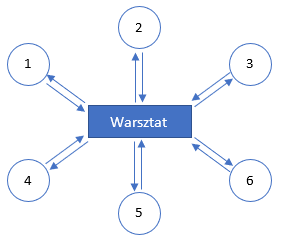
\includegraphics[width = \textwidth]{wykresy/ukl_gniazdowy.png}
\caption{Układ gniazdowy}
\end{subfigure}
\hfill
\begin{subfigure}{0.5\textwidth}
\centering
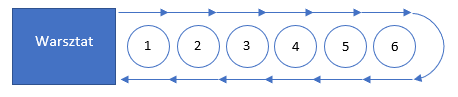
\includegraphics[width = \textwidth]{wykresy/ukl_liniowy.png}
\newline
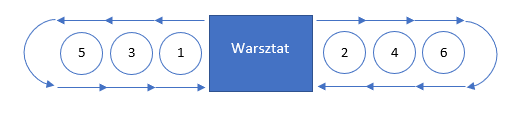
\includegraphics[width = \textwidth]{wykresy/ukl_liniowy_zm.png}
\caption{Układ liniowy standardowy (powyżej) oraz zmodyfikowany (poniżej)}
\end{subfigure}
\end{figure}

\subsection{Struktura modelu}
Zgodnie z~terminologią zastosowaną przez Averilla Lawa (\cite{law}) zastosowany model jest przykładem symulacji zdarzeń dyskretnych (discrete-event simulation). Modelowanymi zjawiskami są: moment wystąpienia awarii dla każdej z maszyn (rozkład wykładniczy) oraz czas naprawy (rozkład Erlanga). Wartości tych zmiennych są losowane niezależnie. Czas oczekiwania na narzędzia oraz czas naprawy maszyny składają się następnie na~czas przestoju maszyny. W~każdej iteracji symulowany jest cały horyzont czasowy (30~dni) dla wszystkich maszyn. Ostateczny wynik jest średnią łącznego czasu przestoju danej maszyny w~kolejnych iteracjach i w~razie potrzeby może być dalej agregowany.

\section{Wyniki analizy}

\begin{table}[ht]
\centering
\label{sr_czas_przestoju}
\caption{Średni czas przestoju (minuty) według układu hali oraz liczby zestawów narzędzi}
\begin{tabular}{l|c|c|c|c|c}
& \multicolumn{5}{|c}{Liczba zestawów narzędzi}\\
układ hali &        1 &       2 &       3 &       4 &       5 \\ \hline
gniazdowy  & 17464.53 & 8360.69 & 8357.60 & 8357.48 & 8357.48 \\
liniowy stand. & 24467.99 & 9770.15 & 9757.19 & 9757.33 & 9757.09 \\
liniowy zmod. & 19646.10 & 8724.11 & 8720.79 & 8719.79 & 8719.80 \\
\end{tabular}
\end{table}

\subsection{Liczba zakupionych zestawów narzędzi}
Wyniki analizy jednoznacznie wskazują, że~w~pierwszej kolejności należy zdecydować o~liczbie zakupionych narzędzi. Zakup drugiego zestawu pozwala ograniczyć czas przestroju o~ponad 50\%. Decyzja ta będzie opłacalna jeśli tylko koszt drugiego zestawu nie~przekroczy równowartości 151.7 godzin przestoju miesięcznie w~przeliczeniu na~maszynę w~układzie gniazdowym bądź 245~godzin w~przypadku układu liniowego (182~godziny dla zmodyfikowanego układu liniowego). Należy zaznaczyć, że~spodziewany koszt zakupu drugiego zestawu narzędzi jest niższy niż dodatkowe nakłady związane z~wdrożeniem układu gniazdowego, a~możliwe do~osiągnięcia korzyści --- znacznie większe. Z~tego powodu rozpoczynamy analizę wyników właśnie od~tego punktu. Co~ważne, zaopatrzenie się w~kolejne zestawy pozostaje prawie bez wpływu na~czas przestoju.

\subsection{Zmodyfikowany układ liniowy}
W~naszej analizie oprócz standardowego układu liniowego rozważamy także jego modyfikację. Prostota rozwiązania sugeruje, że jego wprowadzenie nie powinno nastręczać operacyjnych trudności --- jedyna zmiana względem układu liniowego polega na~przeniesieniu warsztatu do~środka hali, jak na rysunku. W~ten sposób redukcji ulega średnia odległość pomiędzy maszyną, a~warsztatem, a~dzięki temu także czas transportu narzędzi. Tę~ostatnią wielkość oszacowaliśmy na~podstawie specyfikacji podanej dla standardowego modelu liniowego, zakładając proporcjonalną relację między odległością a~czasem transportu. Wyniki symulacji pokazują, że~wdrożenie zaproponowanej przez nas modyfikacji pozwala na~ograniczenie czasu przestoju o~10-20\%. Uznajemy zatem zaproponowaną modyfikację za~zasadną, o~ile tylko jest ona wykonalna operacyjnie.

\subsection{Wybór optymalnego układu maszyn}
Jak zaznaczyliśmy powyżej, zakup drugiego zestawu narzędzi przynosi większą korzyść przy prawdopodobnie niższych kosztach niż modyfikacja układu maszyn. Dalsze zwiększanie liczby dostępnych zestawów nie prowadzi jednak do znaczącego spadku czasu przestoju, konieczne jest wówczas wdrożenie innego schematu hali produkcyjnej. Jak łatwo zauważyć, najlepsze wyniki charakteryzują układ gniazdowy, który jednak wiąże~się prawdopodobnie z~najwyższymi kosztami, z uwagi na konieczność zainstalowania sześciu niezależnych taśmociągów. Zakładając, że~zakupione zostaną dwa zestawy narzędziowe, zmiana układu z~liniowego na~gniazdowy jest opłacalna, o~ile jej koszt nie~przekroczy równowartości 23.5~godziny przestoju miesięcznie w~przeliczeniu na maszynę (6~godzin w~przypadku zmodyfikowanego układu liniowego). Otrzymane liczby są niewielkie, co~wskazywałoby na~niskie prawdopodobieństwo opłacalności takiego rozwiązania, należy jednak pamiętać, że~okres eksploatacji hali produkcyjnej jest najprawdopodobniej bardzo długi.

\section{Analiza wrażliwości}
W~ramach analizy wrażliwości rozważyliśmy dodatkowo trzy scenariusze: możliwość przeprowadzenia dodatkowych szkoleń dla pracowników, które pozwoliłyby ograniczyć czas naprawy, konieczność czasowego wyłączenia z~użycia niektórych maszyn z~powodu spadku popytu oraz zakup maszyn nowej generacji, charakteryzujących się niższą awaryjnością (dłuższy przeciętny czas pracy bez usterki).

\subsection{Szkolenia dla pracowników}
Rozważany przez nas scenariusz zakłada możliwość odpowiedniego przeszkolenia pracowników, które pozwoliłoby ograniczyć przeciętny czas naprawy o~1-4~minuty. Jak widać na wykresie~\ref{wyk_szkolenia}, rozsądne przybliżenie spodziewanego spadku łącznego czasu przestoju powinna zagwarantować funkcja liniowa. Opierając się na tym założeniu wnioskujemy, że zakup szkoleń jest opłacalny tak długo, jak koszt ograniczenia średniego czasu pojedynczej naprawy o~minutę nie przekracza 5.9~godziny przestoju miesięcznie w~przeliczeniu na~maszynę w~układzie liniowym, 6.3~godziny w~układzie gniazdowym oraz 6.4~godziny w~zmodyfikowanym układzie liniowym.
\begin{figure}
\centering
\caption{Przeciętny miesięczny czas przestoju dla~poszczególnych maszyn}
\label{wyk_szkolenia}
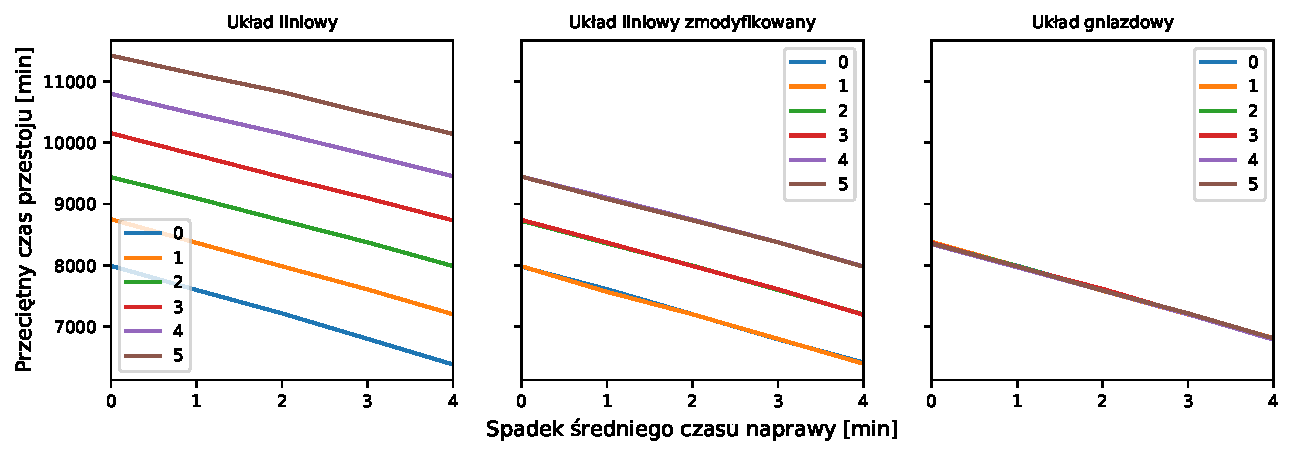
\includegraphics[width = 0.9\textwidth]{wykresy/szkolenia.pdf}
\end{figure}

\subsection{Czasowe wyłączenie maszyn z użytku}
Przejściowy spadek liczby zamówień może wiązać się z~koniecznością czasowego wyłączenia pewnej liczby maszyn z~użytku. Przeprowadziliśmy zatem analizę, która miała za zadanie wyznaczyć optymalny układ w~przypadku gdy efektywnie eksploatowanych jest mniej niż 6~maszyn. Układ liniowy w~swojej standardowej wersji wypada korzystniej od gniazdowego wyłącznie w~przypadku, gdy aktywna jest tylko jedna maszyna --- taki scenariusz należy raczej zakwalifikować jako mało prawdopodobny, ponieważ oznaczałby najprawdopodobniej bardzo znaczące problemy ze zbytem produktów. Przewaga układu gniazdowego maleje w~przybliżeniu liniowo wraz ze spadkiem liczby maszyn pozostających w~użyciu. Warto zauważyć, że zmodyfikowany układ liniowy jest nie~mniej efektywny od~gniazdowego jeśli pracują co~najwyżej 4~maszyny. Należy zatem wziąć pod~uwagę, że jeśli możliwe są przejściowe spadki produkcji, korzyści z~wdrożenia układu gniazdowego mogą okazać~się mniejsze od~spodziewanych, a~w~niektórych okresach schemat ten może okazać~się nawet droższy w~eksploatacji od swoich alternatyw. Dokładne wartości czasu przestoju w~poszczególnych wariantach można prześledzić na~wykresie~\ref{wyk_recesja}.
\begin{figure}
\centering
\caption{Przeciętny miesięczny czas przestoju w~przeliczeniu na~maszynę}
\label{wyk_recesja}
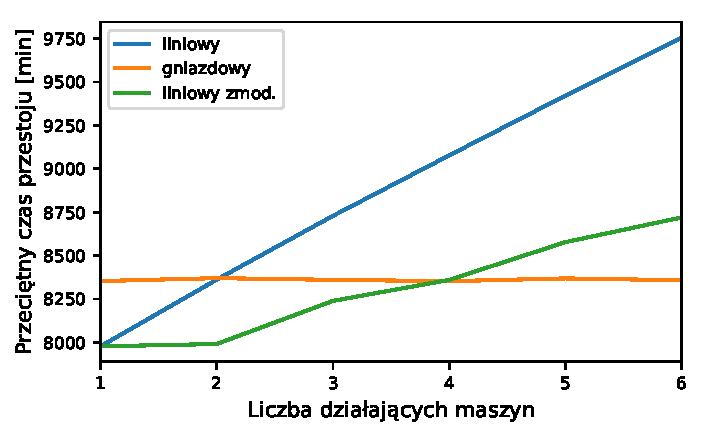
\includegraphics[width = 0.5\textwidth]{wykresy/recesja.pdf}
\end{figure}

\subsection{Zakup maszyn nowszej generacji}
Rozważany scenariusz zakłada zakup sprzętu, który charakteryzuje się niższą awaryjnością, w wyniku czego przeciętny czas pracy maszyn bez usterek jest wydłużony. Przeciętny czas bezawaryjnej pracy maszyny wynosił 75 minut. W naszej analizie został on rozszerzony o~wartości z~przedziału 1-14~minut. Jak widać na wykresie~\ref{wyk_bezawaryjna_praca}, dłuższy czas pomiędzy awariami, a co za tym idzie spadek kosztów, może być odpowiednio przybliżany przez funkcję liniową. Średnia poprawa czasu przestoju maszyny wynosi od 78 do 88 minut (miesięcznie) za każdą dodatkową minutę czasu pomiędzy awariami (dla układu liniowego wynosi 88 minuty, zmodyfikowanego liniowego – 81 minut; gniazdowego – 78 minut).
\begin{figure}
\centering
\caption{Przeciętny czas przestoju dla~poszczególnych maszyn}
\label{wyk_bezawaryjna_praca}
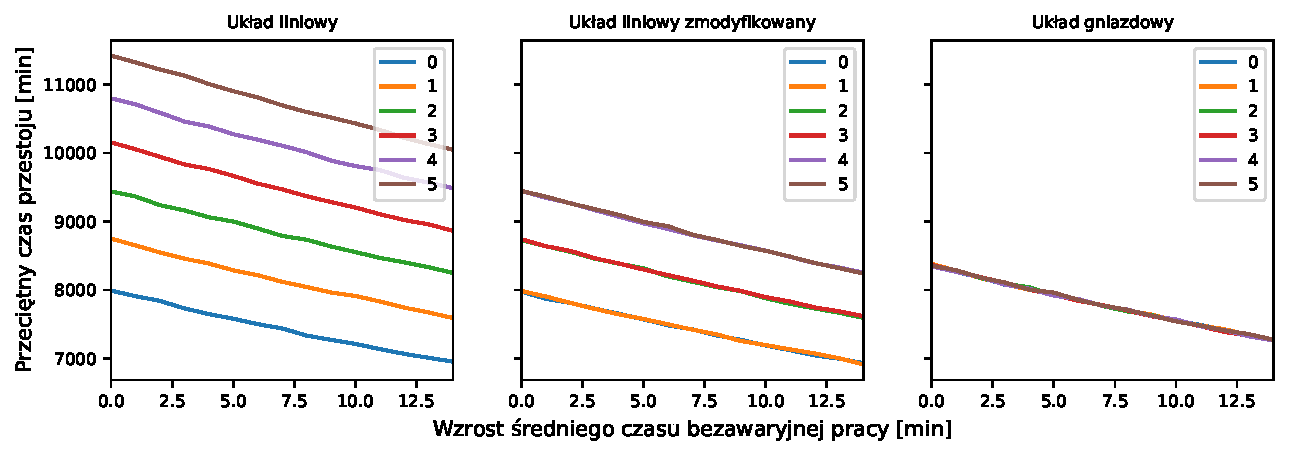
\includegraphics[width = 0.9\textwidth]{wykresy/bezawaryjna_praca.pdf}
\end{figure}

\section{Wnioski}
Podsumowując, rekomendujemy zakup dwóch zestawów narzędziowych do~nowej hali produkcyjnej. Warunkiem opłacalności tej decyzji jest cena pojedynczego zestawu nieprzekraczająca --- zależnie od~wybranego układu --- od~151.7 do~245~godzin przestoju miesięcznie w~przeliczeniu na~maszynę. Jeśli konieczna będzie dalsza redukcja tej wartości, należy rozważyć zmianę układu z~liniowego na~wariant gniazdowy, jednak osiągalne korzyści są w~tym przypadku zauważalnie mniejsze. Rozwiązanie to~będzie tym bardziej atrakcyjne, jeśli istotny jest równomierny rozkład czasu pracy pomiędzy eksploatowanymi maszynami. Jeśli próg opłacalności nie~zostanie spełniony, rekomendujemy wdrożenie zaproponowanej przez nas modyfikacji układu liniowego, która wypada jednoznacznie lepiej od~wersji standardowej, a~w~sytuacji wyłączenia więcej niż 2~maszyn z~użytku generuje niższe koszty niż układ gniazdowy. Analiza wrażliwości wykazała również, że szkolenia przyspieszające usuwanie usterek są opłacalne, gdy koszt skrócenia naprawy o~minutę nie~przekracza wartości ok.~6-godzinnego przestoju w~przeliczeniu na~maszynę miesięcznie, zaś~inwestycja w~maszyny nowszej generacji jest uzasadniona o~ile iloraz różnicy w~cenie oraz różnicy w~czasie bezawaryjnej pracy nie~przekracza kosztu 80-90~minut przestoju miesięcznie. W~obu przypadkach dokładnie wartości zależą od~wdrożonego układu hali produkcyjnej i~zostały zaprezentowane powyżej.


\begin{thebibliography}{9}
%\bibitem{slajdy}
%P.~Szufel, \emph{Zaawansowane Modelowanie Symulacyjne --- materiały do~wykładu}
\bibitem{law}
Averill~M.~Law, W.~David~Kelton,
\emph{Simulation Modeling \& Analysis},
McGraw-Hill, wyd.~piąte, 2015
\bibitem{sayama}
H.~Sayama, \emph{Introduction to the Modeling and Analysis of Complex Systems},
Open SUNY Textbooks, 2015
\bibitem{mielczarek}
Bożena~Mielczarek, \emph{Modelowanie symulacyjne w~zarządzaniu. Symulacja dyskretna},
Oficyna Wydawnicza Politechniki Wrocławskiej, Wrocław~2009
\end{thebibliography}

\end{document}